\documentclass[12pt,a4paper]{article}

\usepackage[utf8]{inputenc}
\usepackage[ngerman]{babel}
\usepackage[T1]{fontenc}
\usepackage{amsmath}
\usepackage{amsfonts}
\usepackage{amssymb}
\usepackage{graphicx}
\usepackage[left=2cm,right=2cm,top=2cm,bottom=2cm]{geometry}
\usepackage{multicol}
\usepackage{booktabs}
\usepackage[hidelinks]{hyperref}
\usepackage{tikz}
\usepackage{pgfplots}
\usepackage{blindtext}
\usepackage{array}
\usepackage{multirow}
\usepackage{bigdelim}
\usepackage{colortbl}
\usepackage{fancyhdr} 
\usepackage{tabularx}
\usepackage{pgfplots}
\usepackage{xcolor}
\usepackage{color}
\usepackage{float}
\usepackage{listings}

\usetikzlibrary{decorations.text}
\usetikzlibrary{tikzmark}
\pagestyle{fancy} 
	\fancyhf{} 
	\fancyhead[L]{
\includegraphics[scale=0.05]{Bilder/dhbw.png}} 
	\fancyhead[C]{\slshape Rechnerarchitektur und Betriebssysteme} 
	\fancyhead[R]{\slshape LaTeX Version}
	\fancyfoot[C]{\thepage}

\usepackage{helvet}
\renewcommand{\familydefault}{\sfdefault}

\newcolumntype{Z}{>{\centering\let\newline\\\arraybackslash\hspace{0pt}}X}
\author{\slshape Robin Rausch, Florian Maslowski, Ozan Akzebe}
\title{Rechnerarchitektur und Betriebssysteme}
\date{\slshape \today}
\begin{document}
\maketitle
\tableofcontents
\newpage
\section{Computerarchitekturen}
	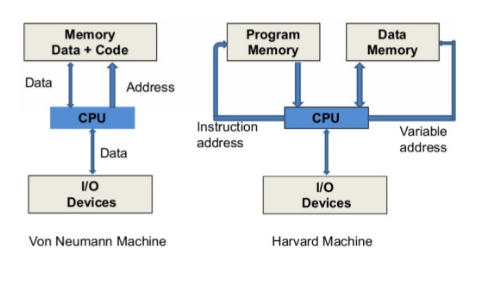
\includegraphics[width=\textwidth]{Bilder/Von-Neuman-Vs-Harvard-Architecture.png}

	\begin{minipage}[t]{0.4\textwidth}
		\subsection{Neumann-Architektur}
		\begin{enumerate}
			\item Ein Adressraum
		\end{enumerate}
	\end{minipage}
	\begin{minipage}[t]{0.55\textwidth}
		\subsection{Harvard-Architektur}
		\begin{enumerate}
			\item Getrennte Adressen für Daten und Code
			\item Getrennte Bussysteme
			\item Kompiliertes Programm nicht ausführbar
			\item gleichzeitige Kommunikation 
		\end{enumerate}
	\end{minipage}

\section{Betriebssysteme Grundlagen}
	\subsection{Architekturen von Betriebssystemen}
		Schnittstelle zwischen der Anwendersoftware und der Speicher- und Prozessverwaltung.
		\begin{description}
			\item[Monolithisches System:] sehr schnell, da alles im Kernel geschieht und es kaum Schnittstellen hat.
			wenn eine Komponente defekt ist, ist der Kernel nichtmehr funktionsfähig. 
			Updates erfodern Gesammtes Update => Größer, zeitintensiver
			\item[Geschichtetes System:] %todo
			\item[Modulares System:]  %todo
			\item[Mirkoarchitektur:] Prozesse dauern länger, da auch Prozesse/Treiber ausgelagert sind
		\end{description}

\section{Binärrechnen}
	\subsection{Komplementbildung}
	\begin{minipage}[t]{0.5\textwidth}
		\subsubsection{Vorzeichenbetragszahl}
			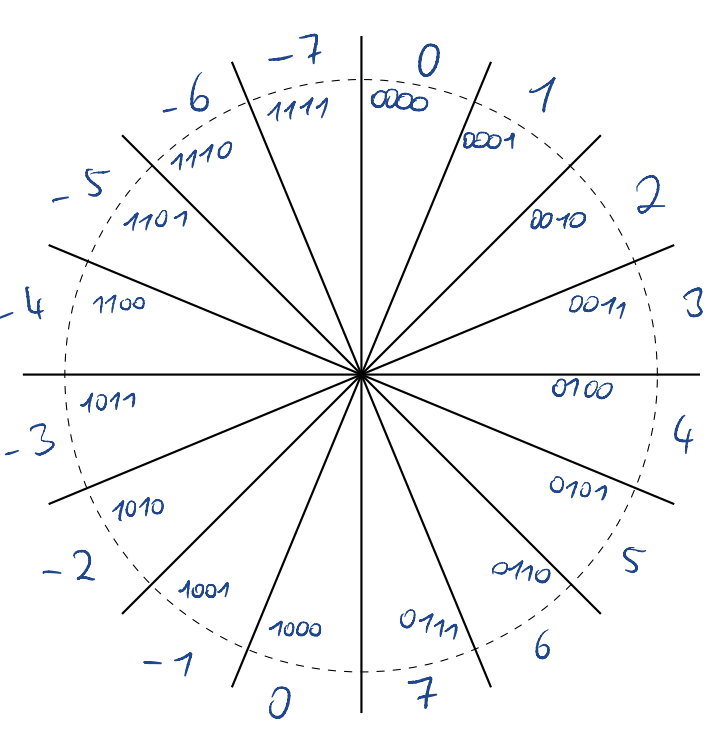
\includegraphics[width=\textwidth]{Bilder/einerkomplement.PNG}
	\end{minipage}
	\begin{minipage}[t]{0.5\textwidth}
		\subsubsection{Zweierkomplement}
			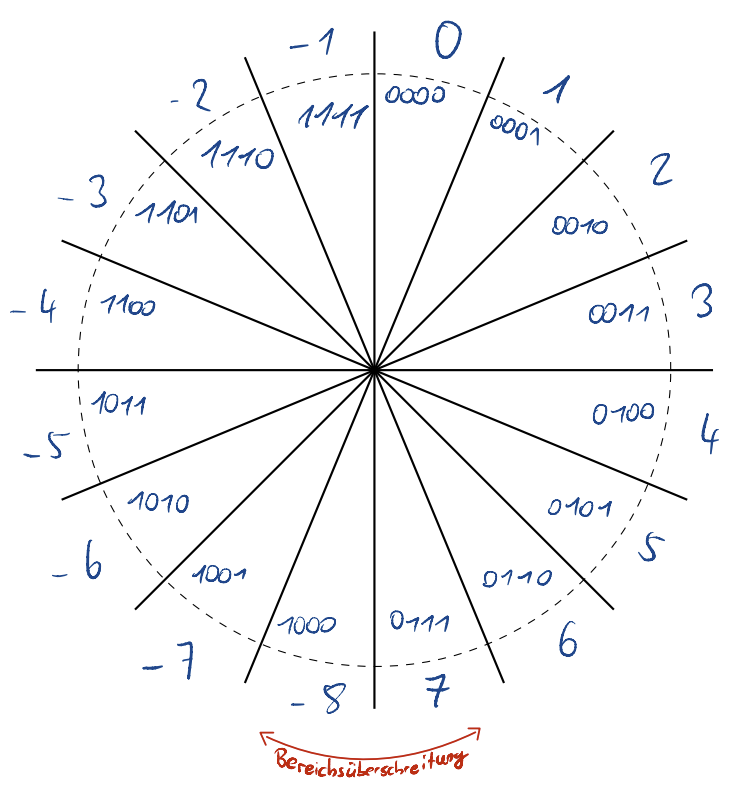
\includegraphics[width=\textwidth]{Bilder/zweierkomplement.PNG}
	\end{minipage}

	\subsubsection{Kommazahlen}
		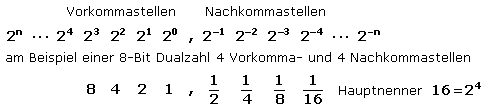
\includegraphics[width=\textwidth]{Bilder/gleitkommazahlen.png}
		
\section{Addierer}
	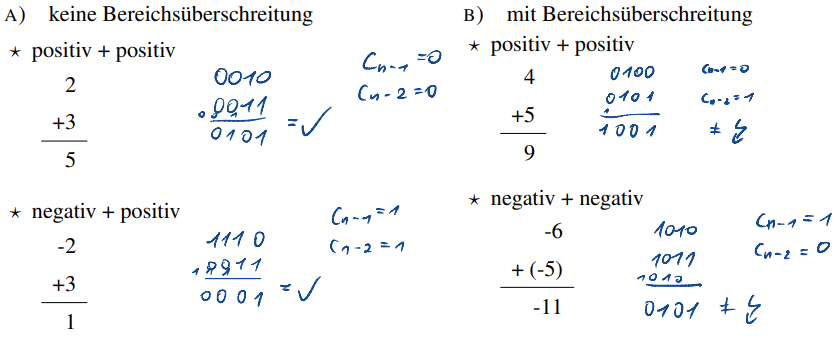
\includegraphics[width=\textwidth]{Bilder/addition.PNG}

	\begin{minipage}[t]{0.5\textwidth}
		\subsection{Halb-Addierer}
		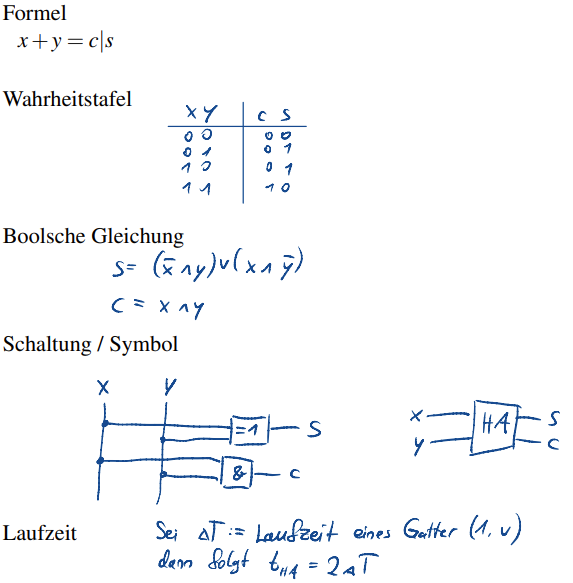
\includegraphics[width=\textwidth]{Bilder/halbaddiere.PNG}
	\end{minipage}
	\begin{minipage}[t]{0.5\textwidth}
		\subsection{Volladdierer}
		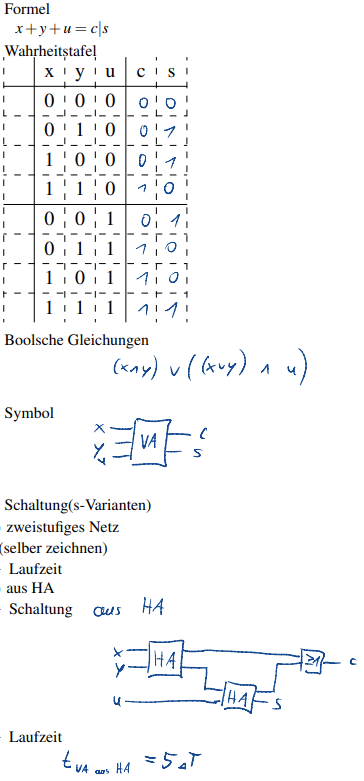
\includegraphics[width=\textwidth]{Bilder/volladdierer.PNG}
	\end{minipage}

	\subsection{N-bit Addierer}
	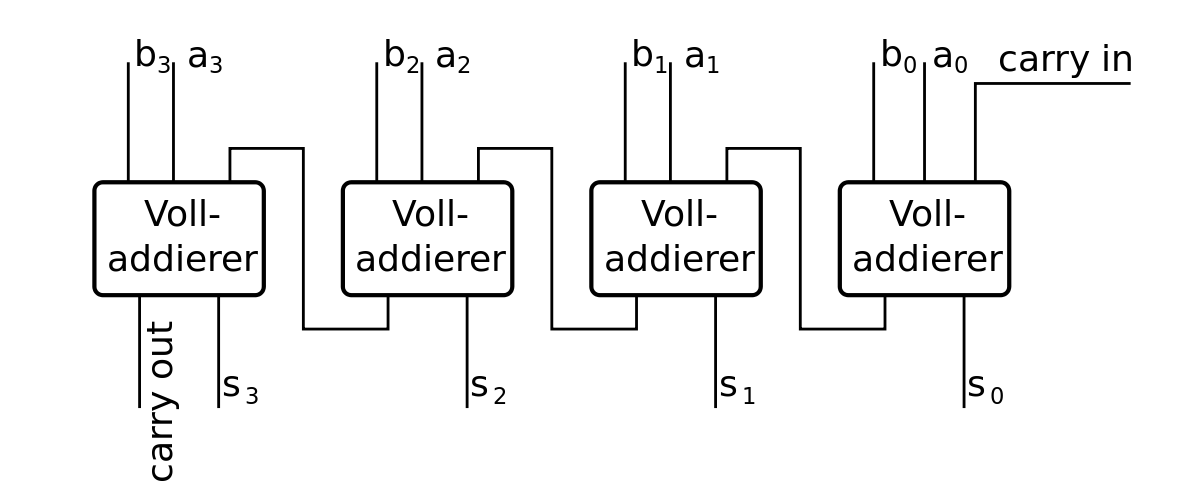
\includegraphics[width=\textwidth]{Bilder/nbitaddierer.png}

	\subsection{Serien Addierer}
	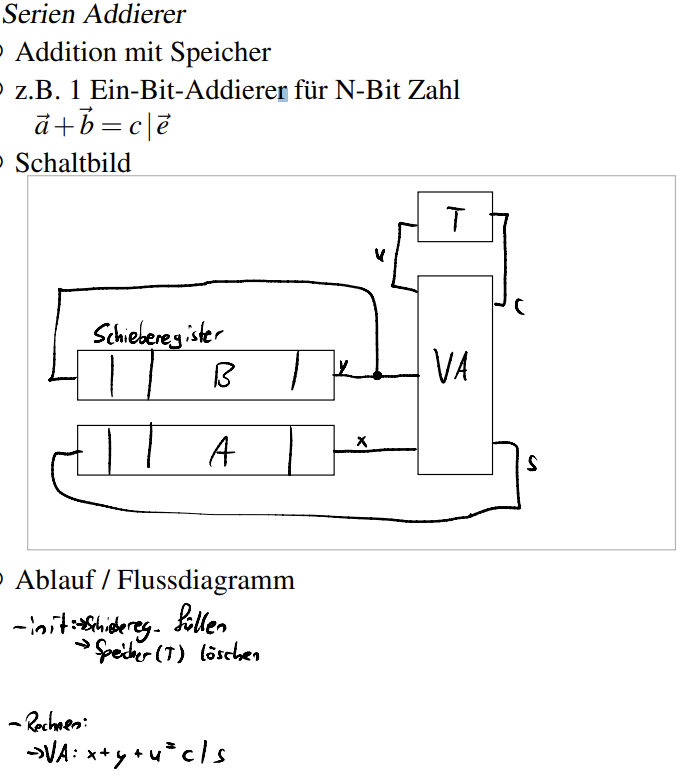
\includegraphics[width=0.6\textwidth]{Bilder/serien_addierer.PNG}

\section{Subtrahierer}
	Das (Zweier-)Komplement der negativen Zahl bilden und mit der anderen addieren.\\
	Die entehende Zahl ist das (Zweier-)Komplement des Ergebnisses.
	\begin{align*}
		&Ohne Komplement:&&Mit Komplement:\\
		&01101 &  &01101\\
		-&01110 & +&10010\\
		\cline{1-4}
		=&11111 & =&11111\\
		\Rightarrow&-00001&\Rightarrow&-00001
	\end{align*}
	
\section{Multiplizieren}
	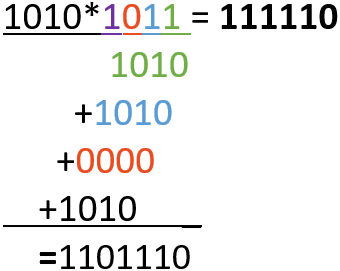
\includegraphics[scale=0.6]{Bilder/BinaryMultiply.png}
	
\section{Dividieren}
	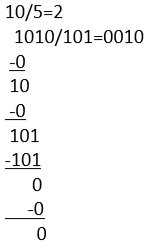
\includegraphics[scale=1.1]{Bilder/BinaryDivision.PNG}
		
\section{Rechnen mit Komplementzahlen}
	\subsection{BCD(=Binary coded decimals)}
		Dezimalziffer wird mit jewweils 4 Bits dargestellt, die zusammen als Tetrade bezeichnet werden. 
		Tetraden im Bereich $ 9<x>16$, werden Pseudotetraden genannt.\\
		Fällt das Ergebnis in den Bereich der 
		Pseudotetraden muss es mit 6 addiert werden.\\
		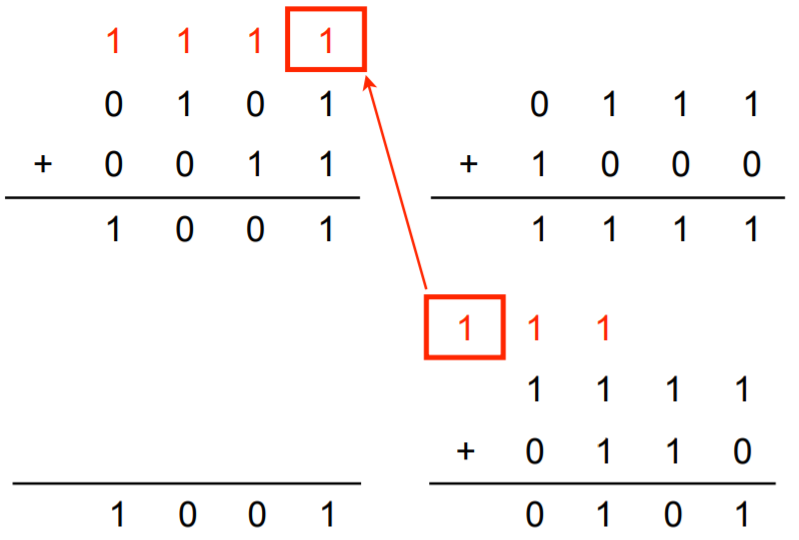
\includegraphics[scale=0.5]{Bilder/BCD-Add.png}

\section{Schaltungen}
	\subsection{Junktoren/binäre Operatoren}
		Nach bindungsstärke sortiert. Klammern binden am stärksten.\\
		\hspace{0.5cm} $\lnot$ NICHT\\
		\hspace{0.5cm} $\land$ UND\\
		\hspace{0.5cm} $\lor$ ODER\\
		\hspace{0.5cm} $\rightarrow$ Implikation\\
		\hspace{0.5cm} $\leftrightarrow$ Äquivalenz\\
		\hspace{0.5cm} $\longmapsto$ Zuweisung\\

	\subsubsection{KV-Diagramm}
		Kästchen bilden, die sich überschneiden dürfen.\\
		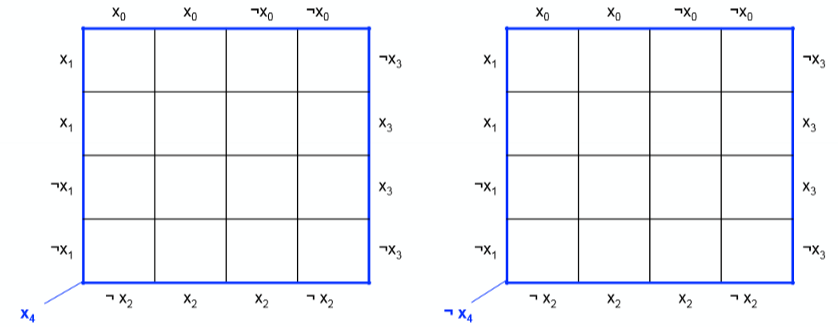
\includegraphics[scale = 0.5]{Bilder/KVDiagramm.png}

	\subsection{Verbindungen:}
		\begin{tabular}{c c c c }
			Keine: & \hspace{0.5cm} Dauerhafte: & Programmierbare (verbindend): & Programmierbar (leitend)\\
			\begin{tikzpicture}
				\draw[-] (0,0) -- (2,0);
				\draw[-] (1,1) -- (1,-1);
			\end{tikzpicture} &
			\begin{tikzpicture}
				\draw[-] (0,0) -- (2,0);
				\draw[-] (1,1) -- (1,-1);
				\draw[fill=black](1,0)circle(2pt);
			\end{tikzpicture} & 
			\begin{tikzpicture}
				\draw[-] (0,0) -- (2,0);
				\draw[-] (1,1) -- (1,-1);
				\draw[-] (0.5,-0.5) -- (1.5,0.5);
			\end{tikzpicture} &
			\begin{tikzpicture}
				\draw[-] (0,0) -- (2,0);
				\draw[-] (1,1) -- (1,-1);
				\draw[-] (0.5,-0.5) -- (1.5,0.5);
				\draw[-] (1.5,-0.5) -- (0.5,0.5);
			\end{tikzpicture}
		\end{tabular}	

\section{Bussystem}
	\textcolor{red}{Hier muss noch Text rein}

\section{Interrupt}
	Die Interrupt-Funktion in Rechnerarchitekturen ermöglicht die Unterbrechung der normalen Programmausführung, um auf Ereignisse zu reagieren, die eine sofortige Aufmerksamkeit erfordern. Ein Interrupt kann beispielsweise durch eine externe Hardwarekomponente wie eine Tastatur oder ein Timer ausgelöst werden. Sobald ein Interrupt auftritt, unterbricht der Prozessor das aktuell ausgeführte Programm und springt zu einer spezifischen Interrupt-Service-Routine (ISR), die den Interrupt behandelt.

	\subsection{Interrupt Controller}
		Der Interrupt-Controller ist eine Hardwarekomponente, die für die Verwaltung von Interrupts zuständig ist. Er empfängt Interrupt-Signale von verschiedenen Quellen und priorisiert sie entsprechend ihrer Wichtigkeit. Der Interrupt-Controller weist jedem Interrupt eine Priorität zu und leitet den Interrupt an den Prozessor weiter, wenn dieser für die Behandlung bereit ist.\\
		Der Interrupt-Controller spielt eine entscheidende Rolle bei der effizienten Verarbeitung von Interrupts in einem Computersystem. Er ermöglicht es, mehrere Interrupts gleichzeitig zu behandeln und sicherzustellen, dass die Interrupts entsprechend ihrer Priorität bearbeitet werden. Durch die Verwendung eines Interrupt-Controllers können Ressourcen effektiv genutzt und Konflikte zwischen verschiedenen Interrupts vermieden werden.

\section{Direct Memory Access - DMA}
	Direct Memory Access (DMA) ist ein Verfahren in Computersystemen, das es bestimmten Geräten ermöglicht, Daten direkt zwischen dem Arbeitsspeicher (RAM) und ihren internen Speicherbereichen auszutauschen, ohne die direkte Beteiligung der CPU.\\
	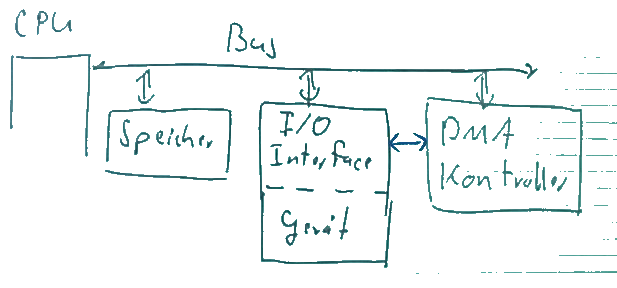
\includegraphics[width=\textwidth]{Bilder/dma-removedBg.png}\vspace{1cm}\\
	\begin{minipage}[c]{0.5\textwidth}
		\textbf{Ablauf ohne DMA:}
		\begin{enumerate}
			\item Quelladresse bestimmen/berechnen
			\item CPU liest von Gerät
			\item Zieladresse bestimmen 
			\item CPU schreibt in Speicher
			\item Zähler erhöhen
			\item Prüfen ob Alles übertragen wurde, ansonsten wiederhole
		\end{enumerate}
	\end{minipage}
	\begin{minipage}[c]{0.5\textwidth}
		\textbf{Ablauf mit DMA:}
		\begin{enumerate}
			\item Kontroller initialisieren
			\item Tansfer anstoßen(programmgesteuert/bedarfsgesteuert)
			\item Übergabe (Kontroller übernimmt)
			\item Transfer (Kontroller steuert(direkt, indirekt))
			\item Kontroller gibt ab (CPU übernimmt Buskontrolle)
		\end{enumerate}
	\end{minipage}

\section{Fließband/Pipeline}
	\includegraphics[width=\textwidth]{Bilder/ohne_fließband.PNG}
	\textbf{Mit Fließband:}\\
	\includegraphics[width=0.4\textwidth]{Bilder/mit_fließband.PNG}		
	
\section{Betriebssysteme}
	Schnittstelle zwischen der Anwendersoftware und der Speicher- und Prozessverwaltung.\\
	
	\begin{figure}[H]
		\centering
		\begin{tikzpicture}
			\def\Radius{2}
			\def\radius{1}
			\begin{scope}[even odd rule]
				\clip[rotate=0.0] (0,0) -- (0:\Radius) arc (0:360:\Radius) --cycle;
				\fill[cyan!60!white] circle[radius=\Radius] circle[radius=\radius];
				\pgfmathsetmacro\bradius{(\radius+\Radius-(\ht\strutbox-\dp\strutbox)/(1cm))/2}
				\path[decoration={text along path,text align={align=center},reverse path,text={Prozess und 								Speicherverwaltung}}, decorate,rotate=-50] (0:\bradius) arc (0:280:\bradius);
			\end{scope}
			\def\Radius{3}
			\def\radius{2}
			\begin{scope}[even odd rule]
				\clip[rotate=0.0] (0,0) -- (0:\Radius) arc (0:360:\Radius) --cycle;
				\fill[cyan!40!white] circle[radius=\Radius] circle[radius=\radius];
				\pgfmathsetmacro\bradius{(\radius+\Radius-(\ht\strutbox-\dp\strutbox)/(1cm))/2}
				\path[
				decoration={text along path,text align={align=center},reverse path,
				text={Kernel}},
				decorate,rotate=-50]
				(0:\bradius) arc (0:280:\bradius);
			\end{scope}
			\def\Radius{4}
			\def\radius{3}
			\begin{scope}[even odd rule]
				\clip[rotate=0.0] (0,0) -- (0:\Radius) arc (0:360:\Radius) --cycle;
				\fill[cyan!20!white] circle[radius=\Radius] circle[radius=\radius];
				\pgfmathsetmacro\bradius{(\radius+\Radius-(\ht\strutbox-\dp\strutbox)/(1cm))/2}
				\path[
				decoration={text along path,text align={align=center},reverse path,
				text={Anwendersoftware}},
				decorate,rotate=-50]
				(0:\bradius) arc (0:280:\bradius);
			\end{scope}
			\draw [line width = 1.5pt](0,0)circle(2);
			\draw [line width = 1.5pt](0,0)circle(3);
			\draw [line width = 1.5pt](0,0)circle(4);
			\filldraw[fill=cyan!80!white, draw=black, line width = 1.5pt](0,0) circle (1);
			\node at (0,0){\small Hardware};
		\end{tikzpicture}
		\caption{Aufbau eines Betriebssystemes}
	\end{figure}

\subsection{Architekturen von Betriebssystemen}
	
\section{Speicheraufbau}

	\textbf{Speichermedien} nach Schnelligkeit sortiert:\\
	Prozessorregister => Prozessorcache => Hauptspeicher => Festplatte\\

	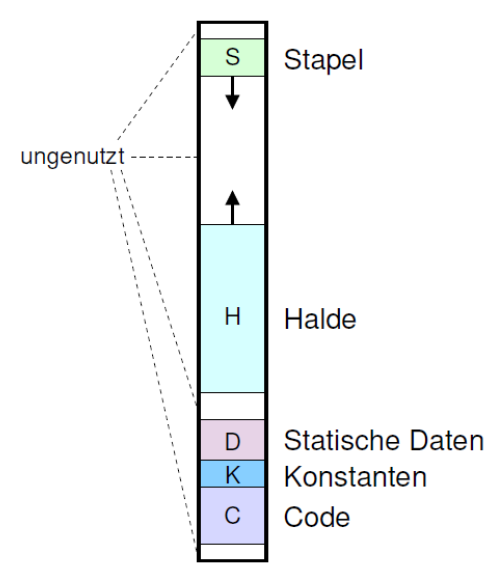
\includegraphics[scale=0.8]{Bilder/Speicheraufbau.png}
	\begin{description}
		\item[Stapel/Stack:] Stapelartige Datenstruktur für Variablen. Nur oberstes Glied kann gelesen oder hinzugefügt/gelöscht(push \& pop) werden.
		\item[Halde/Heap:] Auf Binärbaum basierte Datenstruktur. Dynamische Speicherung von Objekten. Schnell, Effiziente Speichernutzung, simple Verwaltung. Mit malloc Speicher allokieren/reservieren
		\item[Statische Daten:] 
		\item[Konstanten:]
		\item[Code:] 
	\end{description}

\section{Speicherverwaltung und Dateisysteme}
	\subsection{Speicherhierarchie}
		Speicher werden nach ihrer Schnelligkeit in eine Hierarchie eingeordnet, von kurzer zu langer Zugriffszeit.
		\begin{center}
			\begin{tabularx}{13cm}{XXXlXX}
				&&1.& Prozessorregister&&\\
				&&2.& Prozessorcache&&\\
				&&3.& Hauptspeicher&&\\
				&&4.& Festplatte&&\\
				&&5.& Wechseldatenträger&&\\
			\end{tabularx}
		\end{center}

	\subsection{Direkte Speicherverwaltung}
		Beim Einprogrammbetrieb verwaltet das Betriebssystem den Hauptspeicher als einen großen Speicherblock. Dieser besteht aus System und Benutzerbereich.
		\begin{center}
			\begin{tabularx}{13cm}{|X|X|X|}
				\hline
				Betriebssystem&Programm&freier Speicher \\
				\hline
			\end{tabularx}
		\end{center}
		\textit{Problem:}\newline
		Die Programmgröße ist durch die Speichergröße begrenzt. Der Hauptspeicher ist somit zu klein für alle aktiven Prozesse.\newline
		\textit{Lösung: Swapping}

	\subsection{Swapping}
		Beim Swapping wird ein Bereich der Festplatte als sogenannter \textit{'Swap-Space'} deklariert. In diesen können Prozesse ausgelagert werden. Daten und Programmcode des Prozesses werden vollständig in den Swap Space ausgelagert.				
		\begin{center}
			\textbf{Ein ausgelagerter Prozess kann nicht ausgeführt werden.}
		\end{center}
		
		\textbf{Verschiedene Strategien:}
		\begin{description}
			\item[Not resently used] 
			\item[First in, first out]
			\item[Least frequently used]
		\end{description}

		\begin{figure}[h]
			\centering
				\begin{tikzpicture}
					\node (A) at (0,2) [circle,draw,fill=purple!45] {Prozess A};
					\node (B) at (0,-0.7) [circle,draw,fill=orange!50] {Prozess B};
					\draw[black, very thick] (-2,-2) rectangle (2,4);
					\node (D) at (0, 3.6){Hauptspeicher};
					\draw[black, very thick] (4.5,-2) rectangle (8.5,4);
					\node (E) at (6.5, 3.6) {Festplatte};
					\node (C) at (6.5,2) [circle,draw,fill=cyan!50] {Prozess C};
					\draw[->, very thick] (A) to[out=10, in=150] (C);
					\draw[->, very thick] (C) to[out=200, in=-30] (A);
					\node (F) at (6.5, -0.7) [circle,draw,fill=blue!30!white] {Prozess D};
					\draw[->, very thick] (B) to[out=10, in=150] (F);
					\draw[->, very thick] (F) to[out=200, in=-30] (B);
					\node (G) at (3.25,1.4){\textcolor{red}{einlagern}};
					\node (H) at (3.25,3.2){\textcolor{red}{auslagern}};
				\end{tikzpicture}
			\end{figure}
		\begin{center}
			Demnach wären hier nur Prozess A und Prozess B ausführbar.
		\end{center}
		\noindent Ein Prozess wird ausgelagert wenn:
		\begin{itemize}
			\item Ein Prozess, der neu entsteht nicht im Hauptspeicher untergebracht werden kann.
			\item Ein Prozess, seinen Hauptspeicherplatz erweitern möchte, jedoch kein zusätzlicher Speicher verfügbar 					  ist.
			\item Ein \textit{wichtigerer} Prozess aus dem Swap-Space eingelagert werden muss und für ihn kein 							  Hauptspeicherbereich verfügbar ist.
		\end{itemize}

	\subsection{virtueller Speicher}
		\noindent Festplattenspeicher und Hauptspeicher werden zu einem Speicherblock vereint. Dadurch stehen mehr Speicheradressen zur Verfügung, wie tatsächlich im Hauptspeicher vorhanden sind = virtueller Speicher.
		\begin{center}
			\fcolorbox{green!65!black}{white}{\parbox{\linewidth}{Im Gegensatz zum Swapping können beim virtuellen 								Speicher Prozesse auch nur teilweise im Hauptspeicher stehen, während der Rest meist auf dem 							Festplattenspeicher liegt.}}
		\end{center}
		Jedem Prozess wird ein virtueller Speicher geboten, in den alles außer arbeitenden Code und Daten (bleiben im Hauptspeicher) eingelagert wird. Wird von einem Prozess auf den Speicher zugegriffen, verweist die virtuelle Adresse auf eine reelle Adresse des Hauptspeichers. Dieser Verweis geschieht durch die \textit{MMU (Memory Management Unit)}. Befinden sich die Daten in einem ausgelagerten Festplattenblock, wird dieser in den Hauptspeicher eingelagert. \newline
		\begin{figure}[h]
			\centering
			\begin{tikzpicture}
				\draw[black, very thick, fill=purple!45] (-6,0) rectangle (-1,3);
				\draw[black, very thick] (1,0) rectangle (6,3);
				\draw[black, very thick,fill=orange!50] (-6,-1) rectangle (-1,-4);
				\draw[black, very thick] (1,-1) rectangle (6,-4);
				\node (A) at (-4.9,2.5){Prozess A};
				\node (B) at (-4.9,-1.5){Prozess B};
				\draw[black, very thick,fill=white] (-5.8,0.2) rectangle (-4,2);
				\draw[black, very thick,fill=white] (-3.8,0.2) rectangle (-1.2,2);
				\draw[black, very thick,fill=white] (-5.8,-2) rectangle (-4,-3.8);
				\draw[black, very thick,fill=white] (-3.8,-2) rectangle (-1.2,-3.8);
				\node (C) at (-5,1){Code};
				\node (D) at (-5,-3){Code};
				\node (E) at (-2.5,1.75){virtueller};
				\node (F) at (-2.5,1.3){Speicher};
				\node (G) at (-2.5,-2.25){virtueller};
				\node (H) at (-2.5,-2.7){Speicher};
				\node (I) at (-3,-3.25){$B_1$};
				\node (J) at (-2,-3.25){$B_2$};
				\node (K) at (-3,0.7){$A_1$};
				\node (L) at (-2,0.7){$A_2$};
				\node (M) at (3.5,2.5){Hauptspeicher};
				\node (N) at (3.5,-1.5){Festplatte};
				\draw[black, very thick, fill=orange!50] (1.2,0.2) rectangle (5.8,0.9);
				\draw[black, very thick, fill=purple!45] (1.2,1.2) rectangle (5.8,2);
				\draw[black, very thick,fill=purple!45] (1.2,-2) rectangle (5.8,-2.8);
				\draw[black, very thick,fill=orange!50] (1.2,-3) rectangle (5.8,-3.8);
				\node (O) at (3.5,1.6){Prozess $A_1$};
				\node (P) at (3.5,0.55){Prozess $B_2$};
				\node (Q) at (3.5,-2.45){Prozess $A_2$};
				\node (R) at (3.5,-3.45){Prozess $B_1$};
				\draw [->, very thick, orange](J) to[out=10, in=180] (P);
				\draw [->, very thick, orange](I) to[out=320, in=180] (R);
				\draw [->, very thick, purple](K) to[out=300, in=180] (O);
				\draw [->, very thick, purple](L) to[out=300, in=180] (Q);
				\draw [->, very thick, purple](C) to[out=300, in=180] (K);
				\draw [->, very thick, orange](D) to[out=300, in=180] (I);
				\node (X)  at (6,1.5){};
				\node (Y)  at (6,-2.5){};
				\draw [<->, very thick, red](X) to[out=350, in=10] (Y);
				\node (S) at (6,-0.3)[color=red]{auslagern};
				\node (S) at (6,-0.7)[color=red]{einlagern};
			\end{tikzpicture}
		\end{figure}
		\begin{figure}[h]
		\centering
			\begin{tikzpicture}
				\draw[black, very thick, fill=blue!40!white] (-8,0) rectangle (-4,3);
				\draw[black, very thick] (-2,0) rectangle (2,3);
				\draw[black, very thick] (4,0) rectangle (8,3);
				\node (A) at (-6,2.5){Prozessor};
				\draw[black, very thick, fill=white] (-7.8,1.2) rectangle (-4.2,2);
				\draw[black, very thick, fill=white] (-7.8,0.2) rectangle (-4.2,1);
				\node (B) at (-6,1.6){virtuelle Adresse};
				\node (C) at (-6,0.6){MMU};
				\node (D) at (0,1.5){Hauptspeicher};
				\node (E) at (6,1.5){Festplatte};
				\node (F) at (-4,0.6){};
				\node (G) at (-2,0.6){};
				\node (H) at (2,0.6){};
				\node (I) at (4,0.6){};
				\node (J) at (-8,1.6){};
				\node (K) at (-8,0.6){};
				\draw [->, very thick, red](F) to[out=0, in=180](G);
				\draw [->, very thick, red](H) to[out=0, in=180](I);
				\draw [->, very thick, red](J) to[out=180, in=180](K);
			\end{tikzpicture}
		\end{figure}
		\noindent Durch den Einsatz eines Virtuellen Speichers ergeben sich folgende Vorteile:
		\begin{itemize}
			\item Programmbereiche und Datenbereiche sind in ihrer Länge nicht durch die reelle Größe des 									Hauptspeichers begrenzt.
			\item Es können gleichzeitig mehrere Programme ausgeführt werden, deren Gesamtlänge die 										Hauptspeichergröße überschreitet.
		\end{itemize}

	\subsection{segmentorientierter Speicher}
		\noindent Der Adressraum wird in Segmente variabler Größe entsprechend der der logischen Einheiten des Programms unterteilt. Jedem Segment ist ein Speicherbereich im Haupt oder Festplattenspeicher zugeteilt. Die Virtuelle Adresse besteht aus zwei Teilen, der Segmentnummer und dem Offset. Dieser gibt die Position innerhalb des Segments an.
		\begin{figure}[h]
			\centering
			\begin{tikzpicture}
				\draw[black, very thick] (1,0) rectangle (6,3);
				\draw[black, very thick,fill=orange!50] (-6,-4) rectangle (-1,3);
				\draw[black, very thick] (1,-1) rectangle (6,-4);
				\node (A) at (-4.9,2.5){Prozess};
				\draw[black, very thick,fill=white] (-5.8,2) rectangle (-4,-3.8);
				\draw[black, very thick,fill=white] (-3.8,2) rectangle (-1.2,-3.8);
				\node (B) at (-5,1.7){Code};
				\node (C) at (-2.5,1.75){virtueller};
				\node (D) at (-2.5,1.3){Speicher};
				\node (E) at (3.5,2.5){Hauptspeicher};
				\node (F) at (3.5,-1.5){Festplatte};
				\draw[black, very thick, fill=green!60!blue] (1.2,0.2) rectangle (5.8,2);
				\draw[black, very thick,fill=yellow!90!black] (1.2,-2) rectangle (5.8,-3.8);
				\node (G) at (3.5,1.7){Segment 1};
				\node (H) at (3.5,-2.3){Segment 2};
				\node (I) at (-5,1){Write};
				\node (J) at (-5,0.5){Seg.1};
				\node (K) at (-5,0){Offs.2};
				\node (L) at (-5,-1.2){Read};
				\node (M) at (-5,-1.7){Seg.2};
				\node (N) at (-5,-2.2){Offs.0};
				\draw[black, very thick] (-3.7,1) rectangle (-1.3,-1.3);
				\draw[black, very thick] (-3.7,-1.4) rectangle (-1.3,-3.7);
				\node (O) at (-2.5,0.7){Segment1};
				\node (P) at (-2.5,-1.7){Segment2};
				\draw[black, very thick] (-3.7,0.4)--(-1.3,0.4);
				\draw[black, very thick] (-3.7,0.3)--(-1.3,0.3);
				\draw[black, very thick] (-2,0.3)--(-2,-1.3);
				\draw[black, very thick] (-3,0.3)--(-3,-1.3);
				\draw[black, very thick] (-3,-0.2)--(-2,-0.2);
				\draw[black, very thick] (-3,-0.8)--(-2,-0.8);
				\node (Q) at (-2.5,-0.5){1};
				\node (R) at (-2.5,-1.05){2};
				\node (S) at (-2.5,0.05){0};
				\draw[black, very thick] (-3.7,-2)--(-1.3,-2);
				\draw[black, very thick] (-3.7,-2.1)--(-1.3,-2.1);
				\draw[black, very thick] (-2,-2.1)--(-2,-3.7);
				\draw[black, very thick] (-3,-2.1)--(-3,-3.7);
				\draw[black, very thick] (-3,-2.6)--(-2,-2.6);
				\draw[black, very thick] (-3,-3.15)--(-2,-3.15);
				\node (T) at (-2.5,-2.9){1};
				\node (U) at (-2.5,-3.45){2};
				\node (V) at (-2.5,-2.35){0};
				\draw [->, very thick, red](K) to[out=0, in=180](R);
				\draw [->, very thick, red](N) to[out=0, in=180](V);
				\node (W) at (3.5,1){\scriptsize{Reelle Anfangsadresse + Offset}};
				\node (X) at (3.5,0.5){\scriptsize{= tatsächliche Adresse}};
				\node (Y) at (3.5,-3){\scriptsize{Reelle Anfangsadresse + Offset}};
				\node (Z) at (3.5,-3.5){\scriptsize{= tatsächliche Adresse}};
				\node (a) at (1,1.5){};
				\node (b) at (1,-2.5){};
				\draw [->, very thick, red](R) to[out=0, in=180](a);
				\draw [->, very thick, red](V) to[out=0, in=180](b);
			\end{tikzpicture}
		\end{figure}
		\newline
		Der Prozess gibt mit der virtuellen Adresse an, auf welches seiner Segmente und auf welche Position innerhalb dieses Segmentes er zugreifen möchte. Die Umrechnung von virtuellen in reelle Adressen geschieht mit der Segmenttabelle. Jeder Prozess besitzt eine eigene Tabelle. Die Segmenttabelle eines Prozesses enthält für jedes Segment einen Eintrag mit folgenden Informationen:
		\begin{itemize}
			\item Reelle Anfangsadresse des Segments 
			\item Valid-Bit (gibt an, ob sich das Segment auf dem Hauptspeicher oder auf der Festplatte befindet)
			\item Länge des Segments
			\item Zugriffsrechte
		\end{itemize}
		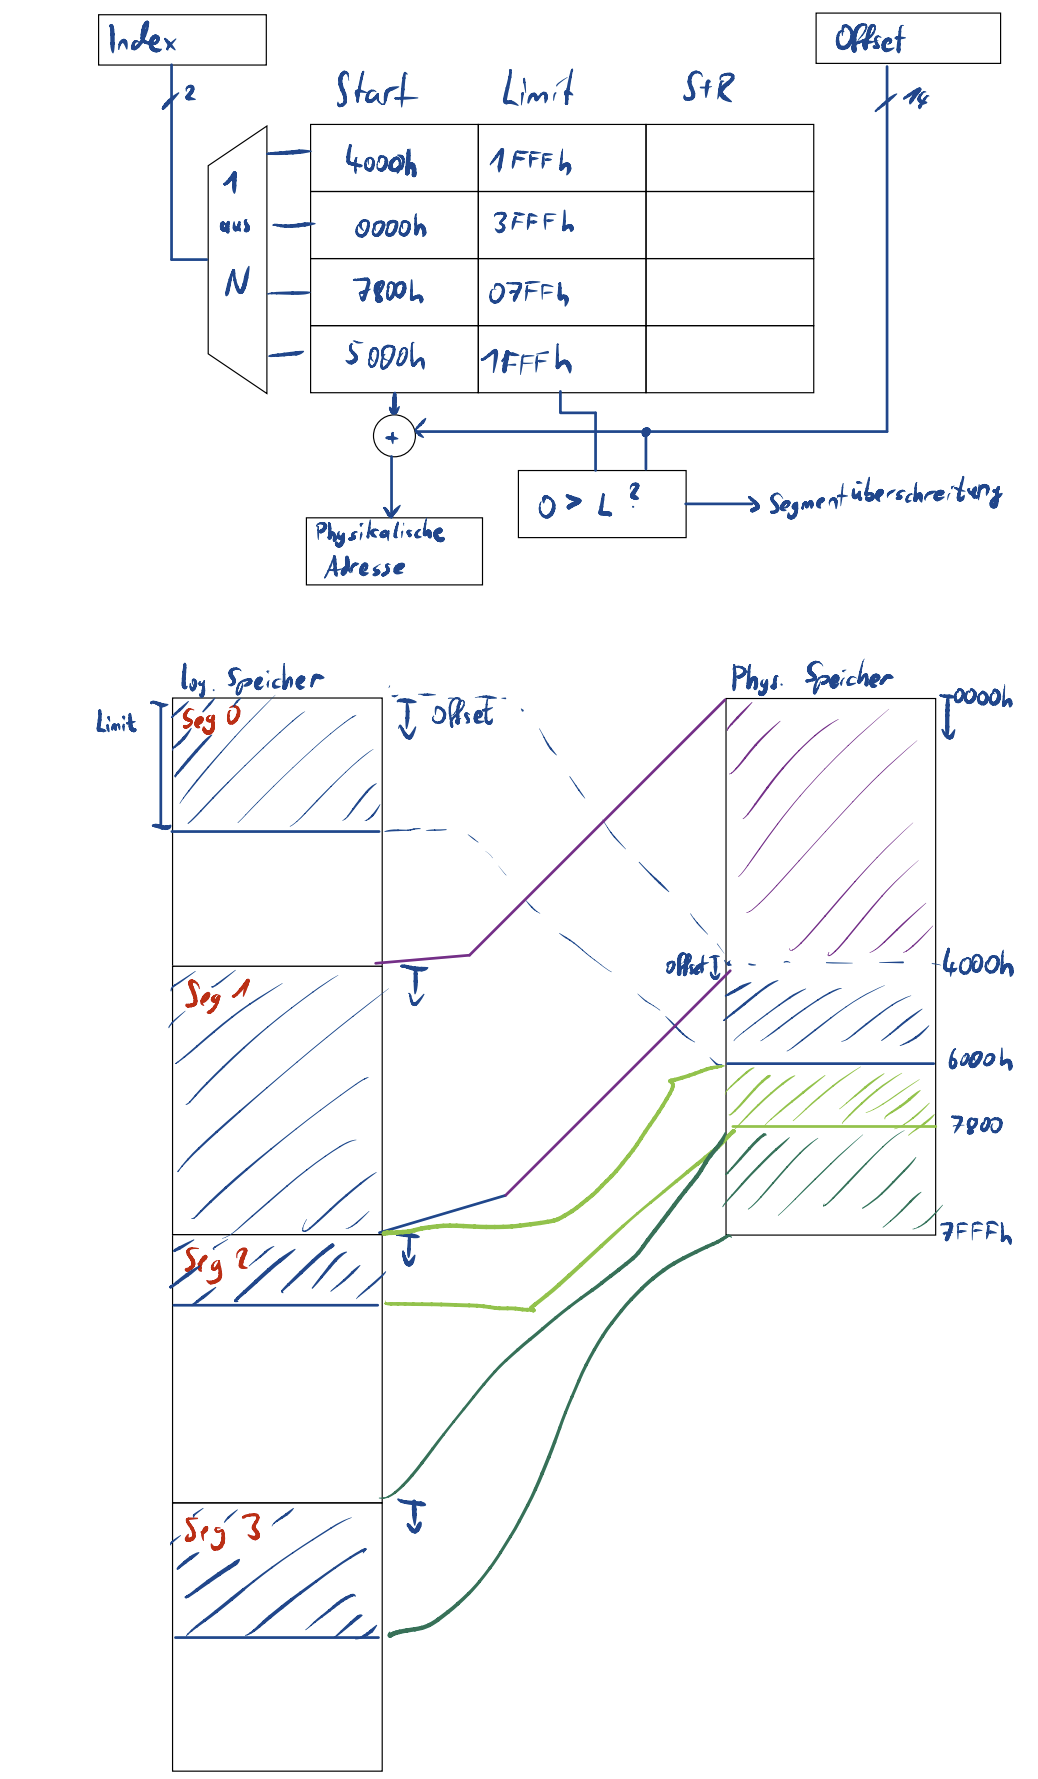
\includegraphics[height=\textheight]{Bilder/segmentorientiert.PNG}
		
	\subsection{seitenorientierter Speicher - \textit{Paging}}
		Strategie zur Speichereinteilung\\
		Speicher wird in gleich große Blöcke/Seiten geteilt\\
		Seitentabelle übersetzt virtuelle in reele Adressen.\\
		Erlaubt es Memory dynamisch zu reservieren.\\
		\begin{center}
			\begin{tabularx}{15cm}{cXllXXc}
				virtuelle Adresse&&&Seitentabelle&&&reelle Adresse \\
			\end{tabularx}
		\end{center}
		\begin{center}
			\begin{tabularx}{13cm}{|r|c|Xl|r|r|Xr|c|l|}
				\hline
				0&2KiB&&&0&RA&&\tikzmark{c-f}&2KiB\cellcolor{yellow}&2048\cellcolor{lime} \\
				\hline
				1&2KiB&&&1&RA&&&2KiB&4096 \\
				\hline
				\cellcolor{lime}2&2KiB\cellcolor{yellow}&\tikzmark{c-g}&&2&\cellcolor{yellow}\tikzmark{c-d}								RA&&&2KiB&6144 \\
				\hline
			\end{tabularx}
		\end{center}
			\begin{center}
				\begin{tabularx}{13cm}{XXXXXXX}
				\end{tabularx}
			\end{center}
		\begin{tikzpicture}[remember picture,overlay,thick,red,shorten <=1pt,shorten >=1pt]
			\begin{scope}[c/.style={shift={(-\tabcolsep,\the\dimexpr\fontdimen22\textfont2\relax)}}]
			\draw[->] ([c]pic cs:c-g) to[bend right] node[below] {verweist} ([c]pic cs:c-d);
			\draw[->] ([c]pic cs:c-d) to[bend left]([c]pic cs:c-f);
			\end{scope}
		\end{tikzpicture}

	\subsection{Demand Paging}
		Hybrid aus Paging und Swapping.\\
		Nicht alle Teile des Prozesses müssen nicht im Memory sein.\\
		Selten genutzte Pages werden ausgelagert.

	\subsection{MMU}
		Die Memory Management Unit übersetzt virtuelle Adressen in Physikalische.\\
		Kontrolliert Speicherzugriffe.\\
		Jeder Prozessor hat eigene MMU.\\
		Für Betriebssysteme mit virtueller Speicherverwaltung (Paging)

	\subsection{Backups}
		Physikalisch getrennte Kopie aktueller Daten.\\
		Hilfreich bei Datenverlust durch zum Beispiel einen System-Virus.\\ 
		Hier wird auf ein Backup zugegriffen, welches vor dem Angriff gemacht wurde.\\

	\subsection{RAID}
		RAID $\neq$ Backup\\
		Für Ausfallsicherheit gibt es verschiedene RAID Systeme, um Daten ausfallsicher zur Verfügung zu stellen.\\
		\begin{description}
			\item[RAID 0:] Speicherung der Daten auf 2 Festplatten für schnellere Zugriffszeiten
			\item[RAID 1:] Redundante Speicherung der Daten auf 2 Festplatten für Ausfallsicherheit
			\item[RAID 5:] Speicherung der Daten mit Paritätsbits auf mehreren Festplatten für kompromiss aus Ausfallsicherheit und verbesserten Zugriffszeiten
			\item[RAID 10:] Beide Systeme(1 \& 0) vereinen 
			\item[RAID 50:] Beide Systeme(5 \& 0) vereinen 
			\item[] ...
		\end{description}
	
	\subsection{FAT}
		Die FAT (\textit{File Allocation Table, Dateizuordnungstabelle}) stellt ein Inhaltsverzeichnis der Festplatte dar und ist notwendig, um die auf dem Datenträger bereitstehenden Daten zu finden. In einem 16-Bit System (FAT 16) sind genau $2^{16} = 65536$ Adressenverwaltungseinträge in der FAT möglich. Bei einer Clustergröße von 512 Byte beträgt die maximale Partitionsgröße 32 MiB ($2^{16} \cdot 512 \text{ Byte}$).
		\begin{figure}[h]
			\centering
			\begin{tikzpicture}
				\fill [olive!40!white](-6,0)rectangle(-4.5,-3);
				\fill [cyan!80!white](-4.5,-1.5)rectangle(0.75,-3);
				\fill [cyan!60!white](-4.5,0)rectangle(-3,-1.5);
				\fill [cyan!40!white](-3,0)rectangle(-1.5,-1.5);
				\fill [cyan!20!white](-1.5,0)rectangle(0.75,-1.5);
				\fill [purple!80!white](0.75,-1.5)rectangle(6,-3);
				\fill [purple!60!white](0.75,-0)rectangle(2.75,-1.5);
				\fill [purple!40!white](2.75,-0)rectangle(4.75,-1.5);
				\fill [purple!20!white](4.75,-0)rectangle(6,-1.5);
				\node at (-5.25,-0.4){Boot};
				\node at (-5.25,-1){Block};
				\node at (-5.25,-1.9){Boot};
				\node at (-5.25,-2.5){Progr.};
				\node at (-2,-2.25){Systembereich};
				\node at (3.25,-2.25){Datenbereich};
				\node at (-3.75,-0.75){FAT};
				\node at (-2.25,-0.5){FAT};
				\node at (-2.25,-1){Kopie};
				\node at (-0.4,-0.5){Root};
				\node at (-0.4,-1){Directory};
				\node at (1.75,-0.75){Cluster 1};
				\node at (3.75,-0.75){Cluster 2};
				\node at (5.375,-0.75){\dots};
				\draw [line width = 1.2pt] (-6,0)rectangle(6,-3);
				\draw [line width = 1.2pt] (-6,-1.5)--(6,-1.5);
				\draw [line width = 1.2pt] (-4.5,0)--(-4.5,-3);
				\draw [line width = 1.2pt] (0.75,0)--(0.75,-3);
				\draw [line width = 1.2pt] (-3,0)--(-3,-1.5);
				\draw [line width = 1.2pt] (-1.5,0)--(-1.5,-1.5);
				\draw [line width = 1.2pt] (2.75,0)--(2.75,-1.5);
				\draw [line width = 1.2pt] (4.75,0)--(4.75,-1.5);
			\end{tikzpicture}
			\caption{Aufbau des FAT Dateisystems}
		\end{figure}\newline
		Durch die geringe Clustergröße können Dateien meist nur fragmentiert abgelegt werden. In einer Dateizuordnungstabelle werden Dateipfade gespeichert und können ausgelesen werden. Das richtige Zusammensetzen der Fragmente ist so möglich.\\
		Ein Nachteil des FAT Systemes liegt darin, dass die FAT an einer festen Position auf dem Datenträger gespeichert ist. Bei Festplatten (Speichermedien mit rotierender Disk und Lesekopf) muss der Lesekopf bei jedem Lese/Schreib Vorgang zur FAT und zurück bewegt werden. Dann muss gewartet werden, bis die FAT den Lesekopf passiert. Das kostet viel Zeit. Heutzutage findet man das FAT System in der Flash Drive Technik.
	
	\subsection{NTFS}
		Das NTFS (\textit{New Technology File System}) Dateisystem wurde erstmals mit Windows NT (\textit{New Technology}) eingeführt und ist seither das preferierte Dateisystem von Windows. NTFS verwaltet Dateien anders als bei FAT in der MFT (\textit{Master File Table}). Diese enthält die sogenannten Records. Zu jeder abgelegten Datei existiert also ein Record in der MFT der folgende Informationen enthält: Header, Informationen (z.B. Erstellungsdatum), den Dateinamen, Zugriffsrechte und die eigentlichen Daten bzw. die Position der Daten im Datenbereich. Dateien kleiner 1.5 KiB können direkt in den Record in der MFT gespeichert werden, wohingegen Dateien größer 1.5 KiB in den Datenbereich des Datenträgers gespeichert werden. Der Record verweist dann auf die entsprechende Stelle. Der Datenbereich ist bei NTFS variabel. Daraus resultieren kürzere Lese/Schreib Zeiten. Außerdem ist die MFT zwei mal zwischen den Datenbereichen enthalten.
		\begin{figure}[h]
			\centering
			\begin{tikzpicture}
				\fill [olive!40!white](-7,0)rectangle(-3,-4);
				\fill [purple!80!white](-3,0)rectangle(-1,-4);
				\fill [cyan!60!white](-1,0)rectangle(1,-4);
				\fill [purple!60!white](1,0)rectangle(3,-4);
				\fill [cyan!40!white](3,0)rectangle(5,-4);
				\fill [purple!40!white](5,0)rectangle(7,-4);
				\draw [line width = 1.2pt](-7,0)rectangle(7,-4);
				\draw [line width = 1.2pt](-7,-1)--(-3,-1);
				\draw [line width = 1.2pt](-5,-1)--(-5,-4);
				\draw [line width = 1.2pt](-3,0)--(-3,-4);
				\draw [line width = 1.2pt](-1,0)--(-1,-4);
				\draw [line width = 1.2pt](1,0)--(1,-4);
				\draw [line width = 1.2pt](3,0)--(3,-4);
				\draw [line width = 1.2pt](5,0)--(5,-4);
				\node at (-5,-0.5){Boot-Block};
				\node [rotate=90] at (-6,-2.5){BIOS Block};
				\node [rotate=90] at (-4,-2.5){Viewers MFT};
				\node [rotate=90] at (-2,-2){Variabler Bereich};
				\node [rotate=90] at (0,-2){MFT};
				\node [rotate=90] at (2,-2){Variabler Bereich};
				\node [rotate=90] at (4,-2){MFT};
				\node [rotate=90] at (6,-2){Variabler Bereich};
			\end{tikzpicture}
			\caption{Aufbau einer NTFS Partition}
		\end{figure}
		\begin{figure}[h]
			\centering
			\begin{tikzpicture}
				\fill [cyan!60!white] (-7,0)rectangle(1,-4);
				\fill [purple!60!white] (1,0)rectangle(7,-4);
				\draw [line width = 1.2pt](-7,0)rectangle(7,-4);
				\draw [line width = 1.2pt](-5,0)--(-5,-4);
				\draw [line width = 1.2pt](-3,0)--(-3,-4);
				\draw [line width = 1.2pt](-1,0)--(-1,-4);
				\draw [line width = 1.2pt](1,0)--(1,-4);
				\node [rotate=90] at (-6,-2){Header};
				\node [rotate=90] at (-4,-2){Informationen};
				\node [rotate=90] at (-2,-2){Dateiname};
				\node [rotate=90] at (0,-2){Rechte};
				\node [rotate=90] at (2,-2){Daten};
			\end{tikzpicture}
			\caption{NTFS Record Dateien kleiner 1.5KiB}
			\end{figure}
			\begin{figure}[h]
			\centering
			\begin{tikzpicture}
				\fill [cyan!60!white] (-7,0)rectangle(1,-4);
				\fill [purple!60!white] (1,0)rectangle(7,-4);
				\draw [line width = 1.2pt](-7,0)rectangle(7,-4);
				\draw [line width = 1.2pt](-5,0)--(-5,-4);
				\draw [line width = 1.2pt](-3,0)--(-3,-4);
				\draw [line width = 1.2pt](-1,0)--(-1,-4);
				\draw [line width = 1.2pt](1,0)--(1,-4);
				\node [rotate=90] at (-6,-2){Header};
				\node [rotate=90] at (-4,-2){Informationen};
				\node [rotate=90] at (-2,-2){Dateiname};
				\node [rotate=90] at (0,-2){Rechte};
				\filldraw [fill=white,line width = 1.2pt](1.2,-0.2)rectangle(6.8,-3.8);
				\fill [purple!20!white] (1.2,-0.2)rectangle(6.8,-1.1);
				\draw [line width = 1.2pt](1.2,-1.1)--(6.8,-1.1);
				\draw [line width = 1.2pt](1.2,-2)--(6.8,-2);
				\draw [line width = 1.2pt](1.2,-2.9)--(6.8,-2.9);
				\draw [line width = 1.2pt](3,-0.2)--(3,-3.8);
				\draw [line width = 1.2pt](4.8,-0.2)--(4.8,-3.8);
				\node at (2.1,-0.7){VCN};
				\node at (3.9,-0.7){LCN};
				\node at (5.8,-0.7){Größe};
			\end{tikzpicture}
			\caption{NTFS Record Dateien größer 1.5KiB}
		\end{figure}\newpage
		\noindent NTFS verfügt über eine hohe Fehlertoleranz. Eine geschriebene Datei wird mit der sich noch im RAM befindender Original Datei verglichen, um Fehler zu vermeiden. Wird ein Fehler erkannt, wird der betreffende Block als fehlerhaft markiert. Der Schreibvorgang wird dann an einem Anderen versucht. Dieses Prinzip nennt man Hot-Fixing. NTFS verfügt zudem über eine sogenannte LOGFILE. Alle Transaktionen werden in diese eingetragen. So kann nach einem Absturz verlorenes Datengut wiederhergestellt werden. NTFS Dateinamen können bis zu 255 Unicode Zeichen lang sein. 
	
	\subsubsection{Dataruns}
		Ist ein Dateneintrag bei NTFS zu groß, muss dieser in den Datenbereich ausgelagert werden, liegt eine sehr große Datei vor, so muss diese zusätzlich fragmentiert werden. Diese Fragmentierung wird mit Hilfe des B-Tree Prinzipes in den Datenbereich des Records eingetragen. Mittles LCN-VCN Mapping ist es nun möglich die fragmentierte Datei auf dem Datenträger richtig und vollständig zusammen zu setzen.

	\subsection{Extended Filesystem}
		Speicherplatz wird in Blöcke zerlegt. Auf diese Blöcke zeigen Inodes. Inodes speichern auch die Attribute und Zugriffsrechte. Alle Informationen zum Dateisystem stehen in einem Superblock. Es gibt mehrere Kopien der Superblöcke.	

\section{Kernel}
	Der Kernel ist die Schnittstelle zwischen der Anwendersoftware und der Speicher- und Prozessverwaltung. Er kann auch als Betriebssystem-Kern bezeichnet werden.
	
	\subsection{Threading}
		\begin{description}
			\item[Multi] Bearbeitet mehrere Threads simultan. Ein Prozess kann mehrere Threads enthalten.
			\item[Hyper] Unterteilt 1 Prozessor in 2 virtulle Prozessoren.
		\end{description}

	\subsection{Kernel}
		
	\subsubsection{Monolithischer Kernel}
		\begin{description}
			\item[+]{sehr schnell, da alles im Kernel geschieht und es kaum Schnittstellen hat}
			\item[-]{wenn eine Komponente defekt ist oder einen Fehler hat, ist der Kernel nichtmehr \\ funktionsfähig}
			\item[-]{Updates müssen im Gesamten direkt erfolgen(z.B. Treiberupdates)}
		\end{description}
		Der Monolitische Kernel wird bei Betriebsystemen wie z.B. DOS, Linux und Android verwendet.
	
	\subsubsection{Mirkokernel}
		\begin{description}
			\item[+]{wenn eine Komponente defekt ist oder einen Fehler hat, kann man den Kernel trotzdem weiterhin 							 verwenden}
			\item[-]{Prozesse dauern länger, da auch Prozesse/Treiber ausgelagert sind}
		\end{description}
		Der Mirkokernel wird bei Betriebsystemen wie z.B. Echtzeitsbetriebssystemen oder RISC OS verwendet.
	
	\subsection{Geschichtetes System}

	\subsection{Modulares System}

	\subsubsection{Hybridkernel}
		\begin{description}
			\item[+]{Nutzung beider Vorteile}
			\item[-]{Nutzung beider Nachteile}
		\end{description}
		Der Hybridkernel wird bei Betriebsystemen wie z.B. Windows oder MAC OS verwendet.

	
\section{Booten}
	Mehrstufiges Starten des Computers. Prüfen ob Hardware passt. OS laden.\\
	\begin{description}
		\item[Kaltstart] Bei Reset oder Stromausfall. Alles laden und prüfen.
		\item[Warmstart] Normal. Hardware wird nicht erneut geprüft.  
	\end{description}

	\subsection{Master Boot Record (MBR)}
		Der Master Boot Record (kurz MBR) enthält ein Startprogramm für BIOS-basierte Computer und eine Partitionstabelle.
		Außerdem werden durch den MBR die Partitionen einer Festplatte eingeteilt. Zudem kann man die Betriebssysteme und Dateisysteme der einzelnen Partitionen herauslesen.\\
		Erster Sektor (512 Byte) auf Festplatte. \\
		Gibt an wie und wo Betriebssystem gespeichert ist, um es in den RAM zu laden/booten (Startprogram).\\
		Sektor besteht aus: Bootloader $\Rightarrow$ Disk-Signatur $\Rightarrow$ Nullbytes $\Rightarrow$ Partitionstabelle $\Rightarrow$ Magic Number (55 AA)
		\begin{table}[h]
			\renewcommand{\arraystretch}{1.5}
			\caption{Partitionstabelleneinträge}
			\vspace{.2cm}
			\begin{tabularx}{\columnwidth}{|c|X|}
				\hline
				\cellcolor{cyan!60!white}Adresse&\cellcolor{cyan!60!white}Inhalt \\
				\hline
				00&80hex = bootfähige Partition \\
				&00hex = nicht bootfähige Partition \\
				\hline
				01&CHS-Eintrag des ersten Sektors \\
				\hline
				04&Typ der Partition (Dateisystem/Partitionsytp) \\
				\hline
				05&CHS-Eintrag des letzten Sektors \\
				\hline
				08&Startsektor nach LBA\\
				\hline
				0C&Anzahl der Sektoren in der Partition \\
				\hline
			\end{tabularx}
		\end{table}
		\begin{table}[h]
		\caption{Master Boot Record}
		\vspace{.2cm}
		\begin{tabularx}{\columnwidth}{|l|X|X|X|X|X|X|X|X|X|X|X|X|X|X|X|X|X|}
			\hline
			\rowcolor{yellow}Offset&0&1&2&3&4&5&6&7&8&9&A&B&C&D&E&F \\
			\hline
			\rowcolor{yellow}0000&eb&48&90&10&8e&d0&bc&00&b0&b8&00&00&8e&d8&8e&c0 \\
			\hline
			\rowcolor{yellow}0010&fb&be&00&7c&bf&00&06&b9&00&02&f3&a4&ea&21&06&00 \\
			\hline
			\multicolumn{17}{|c|}{\dots}\\
			\hline
			\rowcolor{yellow}01a0&10&ac&3c&00&75&f4&c3&00&00&00&00&00&00&00&00&00 \\
			\hline
			\cellcolor{yellow}01b0&\cellcolor{yellow}00&\cellcolor{yellow}00&\cellcolor{yellow}00&\cellcolor{yellow}				00&\cellcolor{yellow}00&\cellcolor{yellow}00&\cellcolor{yellow}00&\cellcolor{yellow}00&\cellcolor{green!				70!blue}00&\cellcolor{green!70!blue}00&\cellcolor{green!70!blue}00&\cellcolor{green!70!blue}00&							\cellcolor{cyan!60!white}00&\cellcolor{cyan!60!white}00&\cellcolor{red!60!white}80&\cellcolor{red!60!					white}01 \\
			\hline
			\rowcolor{red!60!white}01c0&01&00&83&fe&ff&ff&3f&00&00&00&41&29&54&02&\cellcolor{red!50!white}00&						\cellcolor{red!50!white}fe\\
			\hline
			\rowcolor{red!50!white}01d0&ff&ff&82&fe&ff&ff&80&29&54&02&fa&e7&1d&00&\cellcolor{red!40!white}00&						\cellcolor{red!40!white}fe \\
			\hline
			\rowcolor{red!40!white}01e0&ff&ff&83&fe&ff&ff&7a&11&72&02&fa&e7&1d&00&\cellcolor{red!30!white}00&						\cellcolor{red!30!white}fe \\
			\hline
			\rowcolor{red!30!white}01f0&ff&ff&05&fe&ff&ff&74&f9&8f&02&0c&83&6c&04&\cellcolor{purple!50!blue}55&						\cellcolor{purple!50!blue}aa \\
			\hline
		\end{tabularx}
		\textcolor{white}{Abstandhalter}\newline
		\begin{tabularx}{\columnwidth}{XXXXX}
			\cellcolor{yellow}&\cellcolor{green!70!blue}&\cellcolor{cyan!60!white}&\cellcolor{red!60!white}&						\cellcolor{purple!50!blue} \\
			Bootloader&Disk Signatur&Nullbytes&Partitionstabelle&Magic Number \\
		\end{tabularx}
	\end{table}
	
	\subsection{GPT}
		Die Guide Partition Table ist der bessere MBR und hat folgende Vor- und Nachteile gegenüber dem MBR:
		\begin{description}
			\item[+]{Funktioniert auch bei 64-Bit Systemen}
			\item[+]{beliebig viele primäre Partitionen}
			\item[+]{verfügt über Schutz- und Sicherheitsmerkmale(Backups \& Prüfsummen)}
			\item[-]{Nur mit UEFI kompatibel}
		\end{description}
	
	\subsection{UEFI und BIOS}
		UEFI ist das modernere und bessere BIOS. UEFI verfügt gegenüber BIOS folgende Vorteile:
		\begin{itemize}
			\item schnelleres Starten durch paralleles Laden der Treiber
			\item Datenträger können auch mit mehr als 2TB booten
			\item Funktioniert auch bei modernen 64-Bit Systemen
			\item Netzwerke können auch gebootet werden
		\end{itemize}

				
\section{UNIX}
	Mehrbenutzerbetriebsystem.\\
	Arbeitet nach ''Everything is a file'' $\Rightarrow$ Alle Daten liegen als files for.

\section{Prozessverwaltung}
	Die Betriebsmittel des Computersystems müssen zwischen den verschiedenen laufenden Programmen und Systemaufgaben verteilt werden. Zu diesem Zweck werden die einzelnen Aufgaben als Prozesse ausgeführt, die vom Betriebssystem verwaltet werden.
	
	\subsection{Prozesse}
		Ein Prozess besteht aus dem Programmcode und dem Prozesskontext. Der Prozesskontext wiederum setzt sich zusammen aus den Registerinhalten des Prozessors, Speicherbereichen für die Daten und weiteren Betriebsmitteln.\newline
		Ein Programm kann sich aus mehreren Prozessen (Windows: Tasks) zusammensetzen. Ein Prozess kann Unterprozesse besitzen. So ist hier B ein Unterprozess von A, D E und F wiederum sind Unterprozesse von B.
		\begin{figure}[h]
		\centering
			\begin{tikzpicture}
				\filldraw[fill=cyan!60!white, line width=1.2pt](0,0)circle(1cm);
				\node at (0,0) {A};
				\filldraw[fill=orange!60!white, line width=1.2pt](-3,-1)circle(1cm);
				\node at (-3,-1) {B};
				\filldraw[fill=purple!80!white, line width=1.2pt](-5,-1)circle(.5cm);
				\node at (-5,-1) {D};
				\filldraw[fill=purple!60!white, line width=1.2pt](-4.3,-2.5)circle(.5cm);
				\node at (-4.3,-2.5) {E};
				\filldraw[fill=purple!40!white, line width=1.2pt](-2.5,-3)circle(.5cm);
				\node at (-2.5,-3) {F};
				\filldraw[fill=olive!30!cyan, line width=1.2pt](4,-1.5)circle(2cm);
				\node at (5,-0.5) {C};
				\filldraw[fill=olive!20!cyan, line width=1.2pt](3.2,-1)circle(0.85cm);
				\node at (3.2,-1) {Thread1};
				\filldraw[fill=olive!20!cyan, line width=1.2pt](4.5,-2.3)circle(0.85cm);
				\node at (4.5,-2.3) {Thread2};
				\draw [line width=1.5pt] (-0.88,-0.5)--(-2.02,-0.9);
				\draw [line width=1.5pt] (0.88,-0.5)--(2.1,-0.9);
				\draw [line width=1.5pt] (-4.5,-1)--(-4,-1);
				\draw [line width=1.5pt] (-3.6,-1.8)--(-3.95,-2.15);
				\draw [line width=1.5pt] (-2.75,-2)--(-2.6,-2.5);
				\end{tikzpicture}
				\caption{Prozesse, Unterprozesse und Threads}
		\end{figure}
	
	\subsubsection{Threads}
	Prozesse können neben eigenständigen Unterprozessen auch noch Threads haben. Threads sind leichtgewichtige Prozesse innerhalb eines übergeordneten Prozesses. Threads teilen sich mit anderen Threads verschiedene Betriebsmittel. Threads, die dem selben Prozess zugeordnet sind, verwenden den gleichen Adressraum. Dadurch ist eine Kommunikation zwischen diesen Threads möglich.
		\begin{figure}[h]
			\centering
			\begin{tikzpicture}
				\filldraw[fill=olive!30!cyan, line width=1.2pt](4,-1.5)circle(2cm);
				\node at (5,-0.5) {C};
				\filldraw[fill=olive!20!cyan, line width=1.2pt](3.2,-1)circle(0.85cm);
				\node at (3.2,-1) {Thread1};
				\filldraw[fill=olive!20!cyan, line width=1.2pt](4.5,-2.3)circle(0.85cm);
				\node at (4.5,-2.3) {Thread2};
			\end{tikzpicture}
			\caption{Threads in Prozess C}
		\end{figure}
		\begin{description}
			\item[Multi] Bearbeitet mehrere Threads simultan. Ein Prozess kann mehrere Threads enthalten.
			\item[Hyper] Unterteilt 1 Prozessor in 2 virtulle Prozessoren.
		\end{description}
		
	\subsubsection{Prozesszustände}
	Ein Prozess kann folgende Zustände annehmen:
	\subsection{Prozesszustände}
	\begin{enumerate}
		\item Rechnend
		\item Blockiert
		\item Bereit 
		\item Gestartet
		\item Beendet (Suspendiert)
	\end{enumerate}

	\begin{figure}[H]
		\centering
		\includegraphics[width=\textwidth]{Bilder/Prozesszustände.png}
		\caption{Prozessmodell}
	\end{figure}
		
	\subsection{Mehrprozessbetrieb}
	Der Kern eines Prozessors kann immer nur einen Prozess bearbeiten. Prozesse nutzen die zur Verfügung stehende Rechenzeit allerdings nicht optimal, da viele Prozesse auf langsamere äußere Einflüsse warten müssen (bsp. Tastatureingabe). Die Wartezeit eines Prozesses kann effizient genutzt werden, indem diese Wartezeit einem anderen Prozess zugeteilt wird. Man unterscheidet hierbei zwischen zwei Prinzipien:
	\begin{enumerate}
		\item parallel, wenn jeder Kern einer CPU genau einen Prozess bearbeitet
		\item quasiparallel, wenn ein Kern einer CPU mehrere Prozesse nacheinander bearbeitet.
	\end{enumerate}
	\begin{minipage}{.45\textwidth}
		\centering
		\begin{tikzpicture}
		\draw [->](0,0)--(4,0);
		\draw [->](0,0)--(0,2);
		\node [rotate=90] at (-0.5,1){Prozesse};
		\node at (2,-0.4){Zeit};
		\filldraw [fill = cyan!60!white] (0.1,0.1)rectangle(3.8,0.7);
		\filldraw [fill = orange!60!white](0.3,0.8)rectangle(3.3,1.4);
		\end{tikzpicture}\newline
		parallel
	\end{minipage}
	\hspace{1cm}
	\begin{minipage}{.45\textwidth}
		\centering
		\begin{tikzpicture}
		\draw [->](0,0)--(4,0);
		\draw [->](0,0)--(0,2);
		\node [rotate=90] at (-0.5,1){Prozesse};
		\node at (2,-0.4){Zeit};
		\filldraw [fill = cyan!60!white] (0.1,0.1)rectangle(1,0.7);
		\filldraw [fill = orange!60!white](1.1,0.1)rectangle(2,0.7);
		\filldraw [fill = purple!60!white](2.1,0.1)rectangle(3,0.7);
		\end{tikzpicture}\newline
		quasiparallel
	\end{minipage}
	
	\subsection{Multitasking}
	Es wird zwischen zwei Arten von Multitasking unterschieden:
	\begin{enumerate}
		\item Koorperatives Multitasking, hier ist es jedem Prozess selbst überlassen, wann er die Kontrolle an das Betriebssystem zurück gibt. Geringer Verwaltungsaufwand, aber es besteht die Gefahr, dass ein unkoorperativer Prozess das System blockiert.
		\item Präemptives Multitasking, hier steuert das Betriebssystem die Vergabe der Rechenzeit. Der Scheduler kann einem Prozess Zeit oder Ereignis gesteuert Rechenzeit entziehen. Somit ist die Bearbeitung wichtigerer Prozesse zu jedem Zeitpunkt möglich, ein unkoorperativer Prozess legt das System nicht lahm. 
	\end{enumerate}
	
	\subsubsection{Kontext}
	Um einen Prozess unterbrechen zu können, muss dieser nach der Unterbrechung dieselbe Umgebung vorfinden können, welche der Prozess hatte, bevor er unterbrochen wurde. Der Zustand des Prozesses wird also vor der Unterbrechung gespeichert, und bleibt das so lange, bis ihm wieder Rechenzeit zugeteilt wird. Unmittelbar bevor er wieder aktiv wird, wird der gespeicherte Zustand geladen. Aus Sicht des Prozesses scheint es so, als wäre er nie angehalten worden.\newline
	Wichtig für dieses Verhalten ist, dass Prozesse abgeschirmt voneinander sein müssen. Prozess A darf den Kontext von Prozess B nicht kennen. Prozess A erfährt immer nur seinen eigenen Kontext.
	
	\subsection{Scheduling}
	Konkurrieren mehrere Prozesse um die Rechenzeit, teilt der Scheduler ihnen gemäß folgender Kriterien die Rechenzeit zu:
	\begin{enumerate}
		\item \textbf{Fairness}, jeder Prozess erhält einen gerechten Anteil der Rechenzeit
		\item \textbf{Effizienz}, der Prozessor arbeitet möglichst effizient
		\item \textbf{Antwortzeit}, diese wird für interaktiv arbeitende Benutzer minimiert
		\item \textbf{Verweilzeit}, die Wartezeit für die Ausgabe von Stapelaufträgen wird minimiert
		\item \textbf{Durchsatz}, Maximierung der Auftragszahl für ein bestimmtes Zeitintervall
	\end{enumerate}
	
\subsection{Prozess Scheduling Strategien}
Ziel ist möglichst gute Fairness, Effizients, Antwortzeit, Verweilzeit, Durchsatz.

	\subsection{Scheduling Strategien} %% todo ergänzen
		\subsection*{Präemptiv vs. Nicht-Präemptiv}
			\textbf{Präemptiv:} Betriebssystem verwaltet die Prozesse. => Betriebssystem kann dem Prozess Ressourcen bereits vor der Fertigstellung wieder entziehen.\\
			\textbf{Nicht-Präemptiv:} Prozess kann selbst entscheiden wann er Ressourcen freigibt.

		\subsubsection{First Come First Serve}
			Dem Prozess, der als erstes Betriebsmittel und Rechenzeit anfordert, werden diese zugeteilt. \\
			$\longrightarrow$ nicht präemptiv
		
		\subsubsection{Shortest remaining time}
			Prozesse, welche am schnellsten beendet werden können, werden zuerst bearbeitet.\\
			$\longrightarrow$ präemptiv
		
		\subsubsection{Round Robin}
			Jedem Prozess wird gleich viel Rechenzeit in Form von Zeitscheiben zugeteilt. 
			Ist die Zeit abgelaufen, wird der Prozess in den Prozesszustand \textit{bereit} gesetzt, der nächste Prozess wird aufgerufen. 
			Nachdem ein Prozess bearbeitet wurde, und nicht vollständig abgearbeitet werden konnte, wird dieser hinten in der Warteschlange eingereiht, und muss warten, bis er erneut an der Reihe ist. Ein Prozess, der die zugeteilte Rechenzeit nicht in vollem Maße ausschöpfen kann, weil er schon früher fertig ist, blockiert das ganze System, bis die Zeitscheibe abgelaufen ist. Eine effiziente Nutzung der Ressourcen ist daher nicht möglich.\\
			$\longrightarrow$ präemptiv
			
		\subsubsection{Priority}
			Es wird zwischen zwei Priority verfahren unterschieden:
			\begin{enumerate}
				\item \textbf{Präemptiv/ Highest Priority First}\\
						Ein \textit{bereit} stehender Prozess höherer Priorität verdrängt einen \textit{rechnenden} Prozess, geringer Priorität.
				\item \textbf{Nicht Präemptiv}\\
						Prozess mit bester/ Priorität wird zuerst abgearbeitet
			\end{enumerate}
			Bei Prozessen mit gleicher Priorität erfolgt die Abarbeitung nach zum Beispiel Round Robin.\newline\newline
	
\section{Virtualisierung}
	Erstellen einer virtuellen Umgebung.\\
	Unabhängig von tatsächlicher Hardware (solange Hardwareleistung nicht überschritten wird).\\
	
	\subsection{Hypervisor}
		Schicht zwischen Betriebssystemen und Hardware.
		Möglichkeit mehrere Gastsysteme auf einem Hostsystem zu verwalten/hosten.
		Aufgaben: VMs erstellen und ausführen, Ressourcen flexibel verwalten, Abgrenzung von VM-Hardware für Sicherheit.\\
		\begin{description}
			\item[Typ1-Hypervisor:] Bare Metall Hypervisor. Es muss ein physischer Hypervisor gekauft werden.
			\item[Typ2-Hypervisor:] Auf Softwareebene. Ist als Software für Rechner zu erhalten.
		\end{description}
		
\section{Powershell}
	\subsection*{Funktionen}
		\begin{lstlisting}
function addieren ($z1, $z2){
    return $z1 + $z2
}
function subtrahieren ($z1, $z2){
    return $z1 - $z2
}
function multiplizieren ($z1, $z2){
    return $z1 * $z2
}
function dividieren ($z1, $z2){
    return $z1 / $z2
}

$input = Read-Host "What do you want to do? addieren(0), subtrahieren(1), multiplizieren(2), dividieren(3)"

$inputnumber1 = Read-Host "Geben sie ihre erste Zahl ein"
$inputnumber2 = Read-Host "Geben sie ihre zweite Zahl ein"

switch($input){
    0 {$ergebnis = addieren $inputnumber1 $inputnumber2}
    1 {$ergebnis = subtrahieren $inputnumber1 $inputnumber2}
    2 {$ergebnis = multiplizieren $inputnumber1 $inputnumber2}
    3 {$ergebnis = dividieren $inputnumber1 $inputnumber2}
}
Write-Host $ergebnis 
		\end{lstlisting}

	\subsection*{Externe Klassen}

\end{document}